\documentclass{article}
\usepackage[english]{babel}
\usepackage[a4paper, total={6in, 8in}]{geometry}
\usepackage{fancyhdr}
\setlength{\parskip}{0.5em}

% Mathematics packages
\usepackage{amsthm, amsmath, amssymb, amsfonts, nicefrac, mathpazo} 
\usepackage{graphicx}
\usepackage{subcaption}
\usepackage{csquotes}

% Coding colours
\usepackage{color}
\definecolor{codegreen}{rgb}{0,0.6,0}
\definecolor{codegray}{rgb}{0.5,0.5,0.5}
\definecolor{codepurple}{rgb}{0.58,0,0.82}
\definecolor{backcolour}{rgb}{0.95,0.95,0.92}
\definecolor{codeblue}{rgb}{0,0,1}
 
% Coding style
\usepackage{listings}
\lstdefinestyle{mystyle}{
    backgroundcolor=\color{backcolour},   
    commentstyle=\color{codegreen},
    keywordstyle=\color{codeblue},
    numberstyle=\tiny\color{codegray},
    stringstyle=\color{codepurple},
    basicstyle=\footnotesize,
    breakatwhitespace=false,         
    breaklines=true,                 
    captionpos=b,                    
    keepspaces=true,                 
    numbers=left,                    
    numbersep=5pt,                  
    showspaces=false,                
    showstringspaces=false,
    showtabs=false,                  
    tabsize=2
}
\lstset{style=mystyle}

% Easier to call Naturals, Integers and so on.
\newcommand{\N}{\mathbb{N}}
\newcommand{\Z}{\mathbb{Z}}
\newcommand{\Q}{\mathbb{Q}}
\newcommand{\C}{\mathbb{C}}
\newcommand{\ind}{1\hspace{-2.1mm}{1}} %Indicator Function
\newcommand{\I}{\mathtt{i}}
\newcommand{\EE}{\mathbb{E}}
\newcommand{\RR}{\mathbb{R}}
\newcommand{\PP}{\mathbb{P}}
\newcommand{\D}{\mathrm{d}}
\newcommand{\Xe}{X^{\varepsilon}}
\newcommand{\E}{\mathrm{e}}
\newcommand{\Tr}{\mathrm{Tr}}
\newcommand{\HH}{\mathrm{H}}
\newcommand{\sgn}{\mathrm{sgn}}
\newcommand{\atanh}{\mathrm{arctanh}}
\def\equalDistrib{\,{\buildrel \Delta \over =}\,}

% Writing Algorithms
\usepackage[]{algpseudocode}

%%%%%%%%%%%%%%%%%%%%%%%%%%%%%%%%%%%%%%%%%%%%%%%%%%%%%%%%%%%%
\title{M4N9: Project 0}
\author{Yadu Bhageria}
\date{February 2016}

\pagestyle{fancy}
\fancyhf{}
\rhead{CID 00733164}
\lhead{Yadu Bhageria}
\cfoot{\thepage}

%%%%%%%%%%%%%%%%%%%%%%%%%%%%%%%%%%%%%%%%%%%%%%%%%%%%%%%%%%%%
%%%%%%%%%%%%%%%%%%%%%%%%%%%%%%%%%%%%%%%%%%%%%%%%%%%%%%%%%%%%
\begin{document}

\begin{titlepage}
    \begin{center}
    
        Coursework report presented for\\
        M4N9
        
        \vfill
        
        {\Huge Computational Linear Algebra\\ Project 1}
        
        
        \vspace{0.5cm}
        %subtitle?
        
        \vspace{1.5cm}
        
        {\Large Yadu \emph{Bhageria}}
        
        \vfill
        
        Mathematics Department\\
        Imperial College London\\
        United Kingdom\\
        \today
        
    \end{center}
\end{titlepage}
%%%%%%%%%%%%%%%%%%%%%%%%%%%%%%%%%%%%%%%%%%%%%%%%%%%%%%%%%%%%

\tableofcontents
\newpage
%%%%%%%%%%%%%%%%%%%%%%%%%%%%%%%%%%%%%%%%%%%%%%%%%%%%%%%%%%%%

\section{Q1}

The linear system to be solved is

\[
	A u_N = f_N
\]

This can be done by QR factorising $A$ by using the householder triangularization method (given in the house.m file). The output gives a matrix $W$ that contains the Householder reflections and another matrix that is upper triangular, $R$. From this we can compute the matrix, $Q$. This gives

\begin{equation*}
\begin{split}
	A &= QR\\
	A u_N &= QR u_N \\
	R u_N &= Q^\star f_N \\
	R u_N &= b
\end{split}
\end{equation*}

which can be solved using backwards substitution. Note the matrix $Q$ never has to be computed explicitly from $W$ as we can directly compute $Q^\star f_N$ using $W$ and $f_N$.

%%%%%%%%%%%%%%%%%%%%%%%%%%%%%%%%%%%%%%%%%%%%%%%%%%%%%%%%%%%%
\subsection{Algorithm}
So the algorithm used can be written as \\

\begin{algorithmic}
	\State $[m,n] = size(A)$ 
	\Comment{Compute size of A matrix}
	\State $[W,R] =$ house$(A)$
	\Comment{Compute householder reflection and R matrices using house.m}
	\For{$k = 1:n$} \Comment{Compute $ Q^\star b $}
    	\State $b_{k:m} = b_{k:m} - 2 Wb_{k:n,k} ( W_{k:n,k}^\star b_{k:m} )$
	\EndFor
	\For{$i=n:-1:1$} \Comment{Compute $ R^\star b $, i.e. backwards substitution}
   		\State $b_i = \frac{ b_i - R_{i,i+1:n} b_{i+1:n} }{ R_{i,i} }$
	\EndFor
\end{algorithmic}

%%%%%%%%%%%%%%%%%%%%%%%%%%%%%%%%%%%%%%%%%%%%%%%%%%%%%%%%%%%%
\subsection{Results}
Using this code below is the outputted table of errors from the MATLAB code.

\begin{verbatim}
Error_Table = 

     N       Error   
    ___    __________
     16    0.022955
     32    0.0057055
     64    0.0014243
    128    0.00035595
\end{verbatim}

Dividing the errors by $\Delta^2 x$ it can be seen that the errors are indeed decreasing $\sim \Delta^2 x$. This gives

\begin{verbatim}
ScaledError_Table = 

     N     Scaled_Error
    ___    ____________
     16    5.8764      
     32    5.8424      
     64    5.8340      
    128    5.8318      

\end{verbatim}
%%%%%%%%%%%%%%%%%%%%%%%%%%%%%%%%%%%%%%%%%%%%%%%%%%%%%%%%%%%%
%%%%%%%%%%%%%%%%%%%%%%%%%%%%%%%%%%%%%%%%%%%%%%%%%%%%%%%%%%%%
\section{Q2}
%%%%%%%%%%%%%%%%%%%%%%%%%%%%%%%%%%%%%%%%%%%%%%%%%%%%%%%%%%%%
\subsection{Showing given eigenvectors work and finding corresponding eigenvalues}

Eigenvectors $z_k$ with corresponding eigenvalues $\lambda_k$ of $D_2$ will satisfy the following eigenvector-eigenvalue equation. 

\[
	D_2 z_k = \lambda_k z_k \tag{$\star 1$} \label{1}
\]

where $z_k \in \C^N$ and $\lambda_k \in \C$. We can write Eq. \eqref{1} using the given Eq. (2) as

\[
	\frac{z_{k,j+1} - 2 z_{k,j} + z_{k,j-1}}{\Delta x^2} = \lambda_k z_{k,j} \quad \text{for } j = 1 \dots N \tag{$\star 2$} \label{2}
\]

Note $z_{k,j}$ corresponds to the $j^{th}$ entry in the $k^{th}$ eigenvector of $D_2$. Also note that the indices loop around, i.e. $z_{k,1} = z_{k,N+1}$ and $z_{k,0} = z_{k,N}$.

Assume

\[
	z_k = \frac{ 1 }{ \sqrt{N} } \begin{pmatrix}
	\E^{i (k-1) x_1} \\
	\vdots \\
	\E^{i (k-1) x_N}
	\end{pmatrix}
\]

Combining this and $\Delta x = \frac{ 2\pi }{ N }$ and $x_j = (j-1) \Delta x = \frac{ 2\pi }{ N } (j-1)$, the LHS of Eq. \eqref{2} gives

\begin{equation*}
	\begin{split}
		\frac{z_{k,j+1} - 2 z_{k,j} + z_{k,j-1}}{\Delta x^2} 
		& = \frac{\E^{i (k-1) x_{j+1} } - 2 \E^{i (k-1) x_{j} } + \E^{i (k-1) x_{j-1} } }{ \Delta x^2 \sqrt{N} } \\
		& = \frac{\E^{i (k-1) (j) \frac{ 2\pi }{ N } } - 2 \E^{i (k-1) (j-1) \frac{ 2\pi }{ N } } + \E^{i (k-1) (j-2) \frac{ 2\pi }{ N } } }{ \Delta x^2 \sqrt{N} } \\
		& = \frac{ (\E^{i \frac{ 2\pi }{ N } })^{(k-1)(j)} - 2 (\E^{i \frac{ 2\pi }{ N } })^{(k-1)(j-1)} + (\E^{i \frac{ 2\pi }{ N } })^{(k-1)(j-2)} }{\Delta x^2 \sqrt{N}} \\
	\end{split}
\end{equation*}
\begin{equation*}
	\begin{split}
		\intertext{By setting $\omega = \E^{ i \frac{ 2\pi }{ N } }$ it simplifies to}	
		\frac{z_{k,j+1} - 2 z_{k,j} + z_{k,j-1}}{\Delta x^2} 	
		& = \frac{ \omega^{(k-1)(j)} - 2 \omega^{(k-1)(j-1)} + \omega^{(k-1)(j-2)} }{\Delta x^2 \sqrt{N}} \\
		\intertext{Furthermore by setting $\gamma = \omega^{(k-1)} = \E^{ i \frac{ 2\pi }{ N } (k-1) }$ it follows that}
		\frac{z_{k,j+1} - 2 z_{k,j} + z_{k,j-1}}{\Delta x^2} 
		& = [ \gamma - 2 + \gamma^{-1} ] \frac{ \gamma^{(j-1)} }{ \Delta x^2 \sqrt{N}} \\
		& = [ \E^{i (k-1) \frac{ 2\pi }{ N } } - 2 + \E^{-i (k-1) \frac{ 2\pi }{ N } } ] \frac{ \E^{i (k-1) (j-1) \frac{ 2\pi }{ N } } }{ \Delta x^2 \sqrt{N}} \\
		& = \frac{ [2 \cos( (k-1) \frac{2 \pi}{N} ) - 2]}{\Delta x^2} \frac{ \E^{i (k-1) (j-1) \frac{ 2\pi }{ N } } }{\sqrt{N} } \\
		& = \frac{2 [ \cos( (k-1) \frac{2 \pi}{N} ) - 1 ]}{\Delta x^2} z_{k,j} \\
		& = \lambda_k z_{k,j}
	\end{split}
\end{equation*}

Thus satisfying Eq. \eqref{2} proving that the assumed $z_k$'s are indeed eigenvectors of $D_2$ with corresponding eigenvalues $\lambda_k$ given by 

\[
	\lambda_k = \frac{2 [ \cos( (k-1) \frac{2 \pi}{N} ) - 1 ]}{\Delta x^2}
\]

%%%%%%%%%%%%%%%%%%%%%%%%%%%%%%%%%%%%%%%%%%%%%%%%%%%%%%%%%%%%
\subsection{Particular case $k=1$}
For the particular case when $k=1$

\[
	z_1 
	= \frac{ 1 }{ \sqrt{N} } 
	\begin{pmatrix}
	\E^{i (0) x_1} \\
	\vdots \\
	\E^{i (0) x_N}
	\end{pmatrix}
	= \frac{ 1 }{ \sqrt{N} } 
	\begin{pmatrix}
	1 \\
	\vdots \\
	1
	\end{pmatrix}
	\text{ and }
	\lambda_1 = \frac{2 [ \cos( 0 ) - 1 ]}{\Delta x^2} = 0
\]

Thus the LHS of Eq. \eqref{1} gives

\[
	z_1 D_2 = \frac{ 1 }{ \sqrt{N} } 
	\begin{pmatrix}
	1 \\
	\vdots \\
	1
	\end{pmatrix}
	D_2 = \frac{ 1 }{ \sqrt{N} } 
	\begin{pmatrix}
	1-2+1 \\
	\vdots \\
	1-2+1
	\end{pmatrix} = \textbf{0}
\]

the RHS of Eq. \eqref{1} gives

\[
	\lambda_1 z_1 = 0 \cdot z_1 = \textbf{0}
\]

Since LHS $=$ RHS, we have that these satisfy the eigenvalue-eigenvector equation.

%%%%%%%%%%%%%%%%%%%%%%%%%%%%%%%%%%%%%%%%%%%%%%%%%%%%%%%%%%%%
%%%%%%%%%%%%%%%%%%%%%%%%%%%%%%%%%%%%%%%%%%%%%%%%%%%%%%%%%%%%
\newpage
\section{Q3}

Consider two of the eigenvectors of $D_2$, $z_k$ and $z_l$. Then

\begin{equation*}
	\begin{split}
		\langle z_k, z_l \rangle
		& = z_k^\star z_l \\
		& = \frac{1}{N} ( \E^{ -i (k-1) x_1 } , \dots , \E^{ -i (k-1) x_N } )
		\begin{pmatrix}
			\E^{ i (l-1) x_1 } \\
			\vdots \\
			\E^{ i (l-1) x_N }
		\end{pmatrix} \\
		& = \frac{1}{N} \sum_{j=1}^N \E^{ -i (k-1) x_j } \E^{ i (l-1) x_j } \\
		& = \frac{1}{N} \sum_{j=1}^N \E^{ i (l-k) x_j } \\
		& = \frac{1}{N} \sum_{j=1}^N \E^{ i \frac{2\pi}{N} (j-1) (l-k) }\\
		\intertext{Again setting $\omega = \E^{ i \frac{ 2\pi }{ N } }$ it follows that}
		& = \frac{1}{N} \sum_{j=1}^N \omega^{(j-1) (l-k)} \\
		& = \frac{1}{N} [ 1 + \omega^{(l-k)} + \omega^{2 (l-k)} + \dots + \omega^{(N-1) (l-k)} ] \\
		& = 
		\begin{cases}
		    \frac{1}{N} N
		    & \text{ if } k = l \\
		    \frac{1}{N} [ \frac{ \omega^{N (l-k)} - 1 }{ \omega^{(l-k)} - 1 }]
		    & \text{ if } k \neq l
		\end{cases} \\
		\intertext{Note that $\omega^{N(l-k)} = \E^{ i \frac{2\pi}{N} N (l-k) } = \E^{ i 2\pi (l-k) } = 1 \quad \because (l-k) \in \Z$. And so}
		\langle z_k, z_l \rangle 
		& = 
		\begin{cases}
		    1
		    & \text{ if } k = l \\
		    0
		    & \text{ if } k \neq l
		\end{cases} 
	\end{split}
\end{equation*}

Thus $\{ z_k \}$ form an orthonormal basis with respect to the standard inner product.  

%%%%%%%%%%%%%%%%%%%%%%%%%%%%%%%%%%%%%%%%%%%%%%%%%%%%%%%%%%%%
%%%%%%%%%%%%%%%%%%%%%%%%%%%%%%%%%%%%%%%%%%%%%%%%%%%%%%%%%%%%
\newpage
\section{Q4}

The equation to be solved is 

\[
	-\frac{d^2u}{dx^2} = f(x)
\]

which using the second order difference operator, $D_2$, for a periodic function $f(x)$ can be written as a linear system of equations of the form

\begin{equation*}
	- D_2 u_N = f_N \tag{$\star 3$} \label{3}
\end{equation*}

This however does not enforce the zero-mean condition by itself. Thus starting with the decomposition

\[
	D_2 = Z \Lambda Z^{-1}
\]

and noting that 

\[
	Z^{-1} = Z^\star \quad \because \langle z_i, z_j \rangle = \delta_{ij} \implies Z^\star Z = I
\]

Eq. \eqref{3} can be written as

\[
	- D_2 u_N = - Z \Lambda Z^\star u_N = f_N
\]
\[
	\implies  \Lambda Z^\star u_N = - Z^\star f_N
\]

Now writing

\[
	u^{(1)} = Z^\star u_N \quad \text{ and } \quad b^{(1)} = Z^\star f_N
\]

Eq. \eqref{3} gives

\begin{equation*}
	\Lambda u^{(1)} = - b^{(1)} \tag{$\star 4$} \label{4}
\end{equation*}

where $u^{(1)}_1 = z_1 u_N = \frac{1}{\sqrt{N}} \Sigma^{N}_{i=1} u_i = 0$ due to the zero-mean condition and similarly $b^{(1)}_1 = z_1 f_N = \frac{1}{\sqrt{N}} \Sigma^{N}_{i=1} f_i = 0$.

This means that the first equation from linear system of equations given by Eq. \eqref{4}, when enforcing the zero-mean condition, is stating 

\[
	\lambda_1 u^{(1)}_1 = \lambda_1 \cdot 0 = 0 = b^{(1)}_1
\]

This is redundant and thus we can simply ignore it. and solve the other $N-1$ equations. 

This can be done by writing 

\[
	\Lambda^{(-1)} = diag(0, \frac{1}{\lambda_2}, \frac{1}{\lambda_3}, \dots, \frac{1}{\lambda_N})
\]
\[
	\implies u^{(1)} = - \Lambda^{(-1)} b^{(1)} = - \Lambda^{(-1)} Z^\star f_N
\]
\[
	\implies Z^\star u_N = - \Lambda^{(-1)} Z^\star f_N
\]
\[
	\implies u_N = - Z \Lambda^{(-1)} Z^\star f_N
\]

%%%%%%%%%%%%%%%%%%%%%%%%%%%%%%%%%%%%%%%%%%%%%%%%%%%%%%%%%%%%
\subsection{Algorithm}

Given the $Z$ matrix, eigenvalues $\{\lambda_k\}_{k=1:N}$ and the vector $f$ containing values for $f_N$

\begin{algorithmic}
	\State $u = Z^\star f$
	\For{$k = 2:N$}
		\State $u_k = u_k / \lambda_k$
	\EndFor
	\State $u = - Z u$
\end{algorithmic}


%%%%%%%%%%%%%%%%%%%%%%%%%%%%%%%%%%%%%%%%%%%%%%%%%%%%%%%%%%%%
\subsection{Results}

This method gives almost exactly the same error as the previous method.

\begin{verbatim}
Error_Table = 

     N               Error              Real_Error
    ___      ______________________     __________
 
     16     0.022955   - 2.2332e-18i    0.022955
     32     0.0057055  + 6.8926e-18i    0.0057055
     64     0.0014243  - 1.0167e-17i    0.0014243
    128     0.00035595 - 4.8256e-19i    0.00035595
\end{verbatim}

So the error is the same for the real part and there a perturbation on the order of $\epsilon_m$. 

Dividing the errors by $\Delta^2 x$ it can be seen that the errors are indeed decreasing $\sim \Delta^2 x$. This gives

\begin{verbatim}
ScaledError_Table = 

     N         Scaled_Error       Real_Scaled_Error
    ___    __________________     _________________

     16    5.8764 - 5.7169e-16i    5.8764           
     32    5.8424 + 7.058e-15i     5.8424           
     64    5.834  - 4.1646e-14i    5.834           
    128    5.8318 - 7.9062e-15i    5.8318           
\end{verbatim}

%%%%%%%%%%%%%%%%%%%%%%%%%%%%%%%%%%%%%%%%%%%%%%%%%%%%%%%%%%%%
%%%%%%%%%%%%%%%%%%%%%%%%%%%%%%%%%%%%%%%%%%%%%%%%%%%%%%%%%%%%
\newpage
\section{Q5}

The backwards stability conditions that need to be satisfied by the algorithm in part 4 are:

\begin{enumerate}
	\item For the first step of $b^{(1)} = Z^\star f$, the condition is: $$ (Z + \delta Z) \tilde b^{(1)} = f $$ with $\delta Z = Z - \tilde Z$ where $ \| \delta Z \| = \mathcal{O}(\epsilon) $. Note that since Z is unitary, $\| Z \| = 1$.
	\item For the next step of $u^{(1)}_i = b^{(1)}_i / \lambda_i$ for $i = 2:N$ $$ (\lambda_i + \delta \lambda_i) \tilde u^{(1)}_i = \tilde b^{(1)}_i $$ with $ \delta \lambda_i = \lambda_i - \tilde \lambda_i $ where $\frac{\|\delta \lambda_i\|}{\|\lambda_i\|} = \mathcal{O}(\epsilon)$ for $i=2:N$.
	\item For the final step of $u_N = - Z^\star u^{(1)}$ $$ (Z^\star + \delta Z^\star) \tilde u_N = - \tilde u^{(1)} $$ with $\delta Z^\star = Z^\star - \tilde Z^\star$ where $ \| \delta Z^\star \| = \mathcal{O}(\epsilon) $.
\end{enumerate}

Note that the fundamental axion of floating point operations is also valid for complex values numbers with a slightly enlargement adjustment to the value of $\epsilon_m$ \footnote{Numerical Linear Algebra - Trefethen and Bau}. Thus the analysis of complex valued numbers can proceed in exactly the same way as that for real valued numbers.

Step (1) is backwards stable as it is simply a matrix-vector multiplications and such a step also occurs in QR factorization. 

Step (2) is also backwards stable as it simply a floating point operation of a real number with a complex number. Furthermore it is worth noting that $0 < |\lambda_i| \leq \frac{4}{\Delta x^2}$ for $i = 2:N$. So there are no singularities involved and $\lambda_i$ are bounded in magnitude.

Step (3) is also backwards stable as it is the negative of a matrix-vector multiplication. We know that matrix-vector multiplication is backwards stable and taking the negative of values is not a FLOP and thus is also backwards stable.

In lectures it is shown that  the steps involved in using QR factorization to solve a system of equations are backwards stable then therefore so is the entire algorithm. Thus since each of the above steps are backwards stable for the algorithm in Q4 then the entire algorithm should also be backwards stable. 

%%%%%%%%%%%%%%%%%%%%%%%%%%%%%%%%%%%%%%%%%%%%%%%%%%%%%%%%%%%%
%%%%%%%%%%%%%%%%%%%%%%%%%%%%%%%%%%%%%%%%%%%%%%%%%%%%%%%%%%%%
\newpage
\section{Q6}

In pursuit of clarity it is worth mentioning that the operation counts for setting up the problem, computing $\Delta x$, $x$, $f_N$, $A$, $Z$, and $\{ \lambda_k \}_{k=1:N}$ are not included in the following subsections.

Also, complex numbers can be treated as 2 real numbers and thus addition takes 2 FLOPs and multiplication takes 6 FLOPs $\epsilon_{\text{machine}}$.\footnote{Numerical Linear Algebra - Trefethen and Bau}
%%%%%%%%%%%%%%%%%%%%%%%%%%%%%%%%%%%%%%%%%%%%%%%%%%%%%%%%%%%%
\subsection{Part 1 Operation Count}

\begin{enumerate}
	\item From lectures we know that the leading order terms of the number of operations needed for the householder algorithm for a matrix $A \in \RR^{m \times n}$ is $2 m n^2 - \frac{2}{3}n^3$. In this case the operation count is simplified to $2 N^3 - \frac{2}{3}N^3 = \frac{4}{3}N^3$ as $N = n = m$.
	\item $2N^2 + 2N$ FLOPs are needed in the calculation of $Q^\star b$. This is because $2(N - k + 1)$ multiplications are needed and $N - k + 1$ additions and subtractions are needed for $k = 1:N$. i.e. $$ \sum^{N}_{k=1} 4(N - k + 1) = 2N^2 + 2N $$ 
	\item $N^2$ FLOPs are needed for the calculation of $R*^\star b$ i.e. backwards substitution. This is because $N-k$ subtractions and multiplications are needed and 1 division. i.e. $$ \sum_{k=1}^N 2(N-k) + 1 = N^2 $$
\end{enumerate}

In total this gives 

\[
	(\frac{4}{3}N^3) + (2N^2 + 2N) + (N^2) = \frac{4}{3}N^3 + 3N^2 + 2N = \frac{4}{3}N^3 + \mathcal{O}(N^2)
\]

%%%%%%%%%%%%%%%%%%%%%%%%%%%%%%%%%%%%%%%%%%%%%%%%%%%%%%%%%%%%
\subsection{Part 4 Operation Count}

\begin{enumerate}
	\item $4N^2 - 2N$ FLOPs are needed to compute $u^{(1)} = Z^{-1} f_N$. This is becasue there are $2N$ multiplications between a complex and real number and $2(N-1)$ additions ($N-1$ real and complex ones respectively) for each value in the array which is of size $N$. i.e. $$ \sum^{N}_{k=1} 4N - 2 = 4N^2 - 2N $$
	\item $2N - 2$ FLOPs to compute $u^{(2)} = \Lambda^{-1} u^{(1)}$ for rows from $2 /dots N$ where a complex number is being divided by a real number. i.e. $$ \sum^{N}_{k=2} 2 = 2N - 2$$
	\item $8N^2 - 2N$ FLOPS are needed to compute $u_N = Z u^{(2)}$. $6$ computations are needed for a complex and complex number multiplication and there are $N$ such numbers and thus a further $2(N-1)$ additions. This is done $N$ times. i.e. $$ \sum^{N}_{k=1} 2(N - 1) + \sum^{N}_{j=1} 6 =  \sum^{N}_{k=1} 8N - 2 = 8N^2 - 2N $$
\end{enumerate}

Thus the total number of FLOPS needed are

\[
	(4N^2 - 2N) + (2N - 2) + (8N^2 - 2N) = 12N^2 - 2N - 2 = 12N^2 + \mathcal{O}(N)
\]

\subsection{Comparison}

By comparing the theoretical number of FLOPs it is clear than in the limit $N \rightarrow \infty$ the algorithm in part 4 ($\mathcal{O}(N^2)$) should be much faster than the algorithm in part 1 ($\mathcal{O}(N^3)$).

Using the tic and toc functions in MATLAB I get the following results which agree with the theoretical predictions.

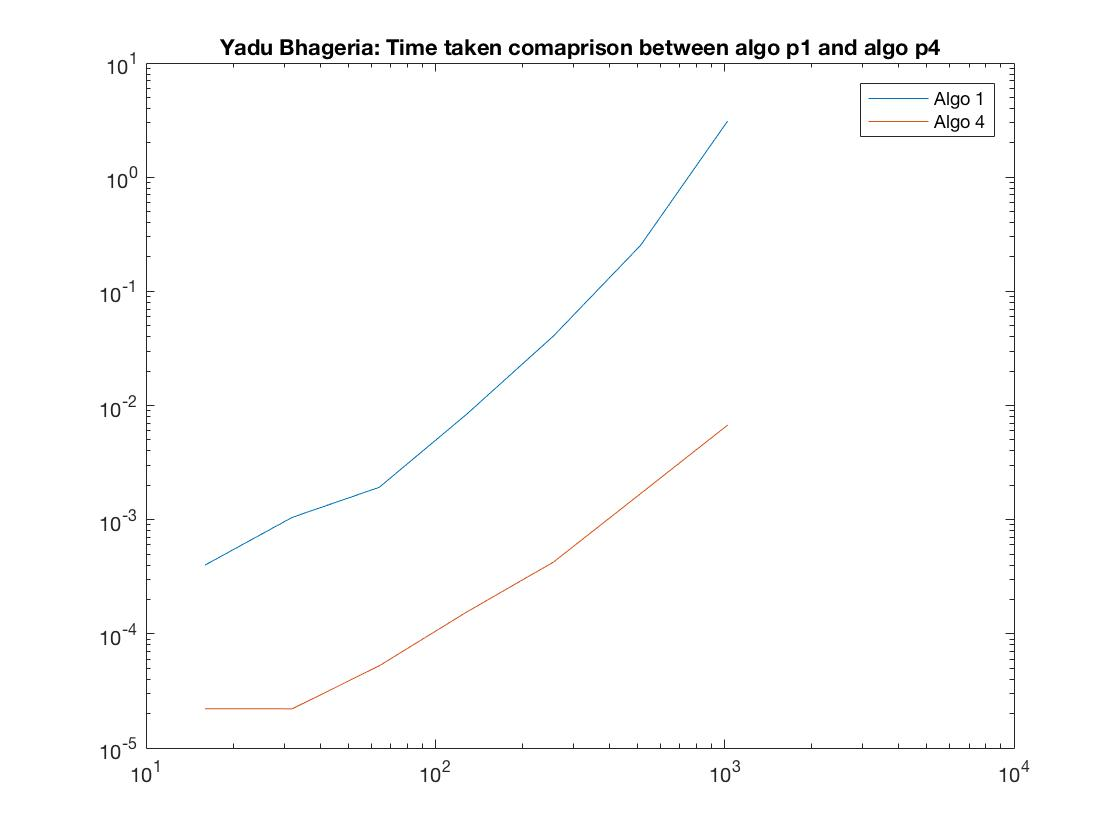
\includegraphics[width = 0.8\textwidth]{fig_timetaken_p1p4.jpg}

%%%%%%%%%%%%%%%%%%%%%%%%%%%%%%%%%%%%%%%%%%%%%%%%%%%%%%%%%%%%
%%%%%%%%%%%%%%%%%%%%%%%%%%%%%%%%%%%%%%%%%%%%%%%%%%%%%%%%%%%%
\newpage
\section{Q7}

The coefficients in the fft() function are precisely those stored in the $Z^\star$ matrix scaled by a factor of $\frac{1}{\sqrt{N}}$. And the coefficients in the ifft() function are precisely those stored in the Z matrix scaled by a factor of $\sqrt{N}$. Since in the algorithm each of Z and $Z^\star$ are applied once the effect cancels out. It is precisely the same as multiplying by $\frac{1}{\sqrt{N}}$ twice due to applying Z and $Z^\star$ and multiplying by $\frac{1}{N}$ in the ifft() function.

Thus the vector matrix multiplication of $ b^{(1)} = Z^\star f_N $ can be replaced by $b^{(1)} =$ fft$(f_N)$ and the vector matrix multiplication of $ u_N = - Z u^{(1)} $ can be replaced by $u_N = -$ ifft$(u^{(1)})$ where $u^{(1)} = \Lambda^{(-1)} b^{(1)} = \Lambda^{(-1)} Z^\star f_N$.

%%%%%%%%%%%%%%%%%%%%%%%%%%%%%%%%%%%%%%%%%%%%%%%%%%%%%%%%%%%%
\subsection{Algorithm}
This gives the new algorithm as

\begin{algorithmic}
	\State $u = $ fft$(f)$
	\For{$k = 2:N$}
		\State $u_k = u_k / \lambda_k$
	\EndFor
	\State $u = -$ ifft$(u)$
\end{algorithmic}

%%%%%%%%%%%%%%%%%%%%%%%%%%%%%%%%%%%%%%%%%%%%%%%%%%%%%%%%%%%%
\subsection{Comparison}

%%%%%%%%%%%%%%%%%%%%%%%%%%%%%%%%%%%%%%%%%%%%%%%%%%%%%%%%%%%%
\subsubsection{Error}

The error remains the same using this method with a perturbation on the order of $\epsilon_m$

\begin{verbatim}
Error_Table = 

     N              Error               Real_Error
    ___     ______________________      __________

     16     0.022955   + 3.9011e-30i    0.022955
     32     0.0057055  - 7.8687e-29i    0.0057055
     64     0.0014243  + 7.4363e-18i    0.0014243
    128     0.00035595 - 1.7416e-17i    0.00035595
\end{verbatim}

\begin{verbatim}
ScaledError_Table = 

     N         Scaled_Error       Real_Scaled_Error
    ___    __________________    _________________

     16    5.8764 + 9.9867e-28i     5.8764           
     32    5.8424 - 8.0576e-26i     5.8424           
     64    5.834  + 3.0459e-14i     5.834           
    128    5.8318 - 2.8535e-13i     5.8318    
\end{verbatim}

%%%%%%%%%%%%%%%%%%%%%%%%%%%%%%%%%%%%%%%%%%%%%%%%%%%%%%%%%%%%
\subsubsection{Runtime Comparison}

Number of operations needed for the Fast Fourier Transform algorithm will be $\mathcal{O}(N\log N)$. fft() and ifft() increase $\mathcal{O}(N\log N)$ as N increases and doing $u_k = u_k / \lambda_k$ increase $\mathcal{O}(N)$ as N increases.

As can be seen, the algorithm utilizing Fast Fourier Transforms is much faster the the previous two algorithms and increases on a smaller order than either of them.

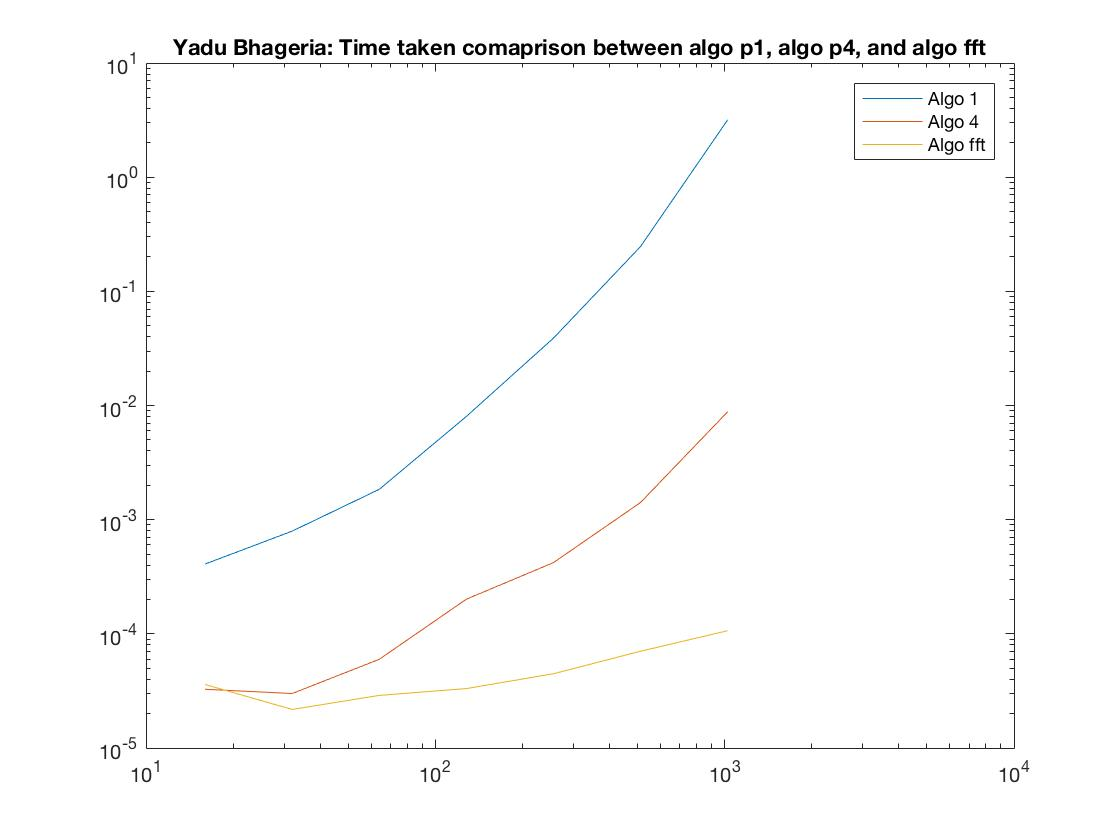
\includegraphics[width = 0.8\textwidth]{fig_timetaken_all.jpg}

%%%%%%%%%%%%%%%%%%%%%%%%%%%%%%%%%%%%%%%%%%%%%%%%%%%%%%%%%%%%
%%%%%%%%%%%%%%%%%%%%%%%%%%%%%%%%%%%%%%%%%%%%%%%%%%%%%%%%%%%%
\newpage
\section{Appendix}

\subsection{Code}
All the code used for this project is submitted with it on blackboard. Here I outline what files are needed for each part. 

\subsubsection{Q1}
The algorithm and implementation in Q1 uses the house.m, construct\_A.m, algo\_p1.m and error\_p1.m files. The error\_p1.m file is the script that produces the error tables and can also produce a plot of the various estimations.

\subsubsection{Q4}
The algorithm and implementation in Q4 uses the construct\_Z.m, construct\_lambda.m, algo\_p4.m and error\_p4.m files. The error\_p4.m file is the script that produces the error tables and can also produce a plot of the various estimations.

\subsubsection{Q6}
The plot producing file timetaken\_p1p4.m calls the time\_p1p4algos.m which in turn calls house.m, construct\_A.m, algo\_p1.m, construct\_Z.m, construct\_lambda.m, and algo\_p4.m files.

\subsubsection{Q7}
The algorithm and implementation in Q7 uses construct\_lambda.m, algo\_fft.m and error\_fft.m files with the latter being the script producing error tables.

The plot producing file timetaken\_all.m calls the time\_allalgos.m which in turn calls house.m, construct\_A.m, algo\_p1.m, construct\_Z.m, construct\_lambda.m, algo\_p4.m, and algo\_fft.m files.

\end{document}

